\newcommand\figlength{6cm}

\chapter{\label{cha:qe_multilingual}Multilingual Quality Estimation with TransQuest}

Machine translation quality estimation is traditionally framed as a supervised machine learning problem \autocite{kepler-etal-2019-openkiwi,lee-2020-two} where the machine learning models are trained on language specific data for quality estimation. We refer to these models as bilingual QE models. This process would require having annotated QE data for all the language pairs. Furthermore, this language specific supervised machine learning process would result in having machine learning models for each language pair separately. 

This traditional approach has obvious drawbacks. As we mentioned before this process requires training data for each language pair. However, the training data publicly available to build QE models is limited to very few language pairs, which makes it difficult to build QE models for many languages. Furthermore, from an application perspective, even for the languages with resources, it is difficult to maintain separate QE models for each language since the state-of-the-art neural QE models are large in size \autocite{ranasinghe-etal-2020-transquest}. 

To understand the scale of this, consider a real-word application where it is required to build a quality estimation solution for European Parliament. European Parliament has 24 languages which would result in 24*23 language pairs which is equal to 552 language pairs. A traditional bilingual QE solution would require 552 training datasets to train the models which is highly challenging and costly to collect and annotate. Furthermore, this would require having 552 machine learning models. State-of-the-art QE models like TransQuest are at least 2GB in size. Having 2GB sized 552 models in the RAM at inferencing time would not be practical. The solution to all these problems is Multilingual QE models. 

Multilingual models allow training a single model to perform a task from and/or to multiple languages. Even though multilingual learning has been applied to many tasks \autocite{ranasinghe-zampieri-2020-multilingual,ranasinghe-zampieri-2021-mudes} including NMT \autocite{nguyen-chiang-2017-transfer, aharoni-etal-2019-massively}, multilingual approaches have been rarely used in QE \autocite{sun-etal-2020-exploratory}. Therefore, in this chapter we explore multilingual models with the \textit{TransQuest} architectures we introduced in Chapters \ref{cha:qe_transquest} and \ref{cha:qe_word} for sentence-level QE and word-level QE respectively. Since we used a crosslingual transformer model that supports 104 languages \autocite{conneau-etal-2020-unsupervised} it was possible to explore multilingual learning with the same setup.


Usually, neural machine learning models are \textit{hungry for data}. They need a lot of annotated data for the training process which can be a challenge for the low resource languages. Recently, researches are trying to exploit this behaviour with learning paradigms such as few-shot and zero-shot learning.  What we define as few-shot learning in this Chapter is the process where the QE model only sees a few examples from a certain language pair in the training process \autocite{10.1145/3386252} while in zero-shot learning, QE model would not see any examples from a certain language pair \autocite{10.5555/1620163.1620201} in the training process. Even though few-shot and zero-shot learning has been popular in machine learning applications including NLP, they have not been explored with QE. Exploring them would be beneficial for the low resource languages which the QE training data is difficult to find. Therefore, in this Chapter, we inspect how the bilingual and multilingual QE models behave in few-shot and zero-shot learning environments.


As far as we know, this is the first study done on multilingual word-level and sentence-level QE. We address three research questions in this chapter:

\textbf{RQ1:} Do multilingual models based on existing state-of-the-art sentence-level and word-level QE architectures perform competitively with the related bilingual models?

\textbf{RQ2:} How does the bilingual and multilingual models perform in a zero-shot environment and what is the impact of source-target direction, domain and MT type for zero-shot learning?

\textbf{RQ3:} Do multilingual QE models perform better with a limited number of training instances (Few-shot learning) for an unseen language pair?


The main contributions of this Chapter are, 

\begin{enumerate}

\item We explore multilingual, sentence-level and word-level quality estimation with the proposed architectures in \textit{TransQuest}. We show that multilingual models are competitive with bilingual models.

\item We inspect few-shot and zero-shot sentence-level and word-level quality estimation with the bilingual and multilingual models. We report how the source-target direction, domain and MT type affect the predictions for a new language pair.

\item The code and the multilingual pre-trained models of \textit{TransQuest} are publicly available to the community\footnote{The pre-trained multilingual QE models are available on HuggingFace model repository on \url{https://huggingface.co/TransQuest}}.

\end{enumerate} 

The rest of this chapter is organised as follows. Section \ref{sec:multilingual_method} discusses the methodology and the multilingual experiments done with 15 language pairs in both aspects of sentence-level QE and word-level QE.  Section \ref{sec:multilingual_results} shows the results and Sections \ref{sec:multilingual_zeroshot} and provide \ref{sec:multilingual_fewshot} further analysis on zero-shot and few-shot learning. The chapter finishes with conclusions and ideas for future research directions in multilingual QE.
 

\section{Methodology}
\label{sec:multilingual_method}
As we mentioned before, we conducted the experiments with the architectures we explored in Chapters \ref{cha:qe_transquest} and \ref{cha:qe_word}. For sentence-level experiments, we used \textit{MonoTransQuest} architecture introduced in Chapter \ref{cha:qe_transquest} which outperformed other open source QE frameworks and best systems submitted to shared tasks in majority of the language pairs and can be considered as the current state-of-the-art in sentence-level QE. For multilingual experiments, we considered both aspects of sentence-level QE; HTER and DA with the datasets introduced in Chapter \ref{cha:qe_introduction}. On the other hand, for word-level experiments we used  the \textit{MicroTransQuest} architecture which again outperformed other open source QE frameworks and best systems submitted to shared tasks in majority of the language pairs in word-level QE. For word-level QE data we considered all the word-level QE datasets introduced in Chapter \ref{cha:qe_introduction}.

For the experiments we considered XLM-R large model and did not use the ensemble models to keep the multilingual experiments simpler. We applied the same set of configurations for all the training processes in order to ensure consistency between all the experiments. We used a batch-size of eight, Adam optimiser and a linear learning rate warm-up over 10\% of the training data. During the training process, the parameters of XLM-R-large model, as well as the parameters of the subsequent layers, were updated. The models were trained using only training data. Furthermore, they were evaluated while training once in every 100 training steps using an evaluation set that had one fifth of the rows in training data. We performed early stopping if the evaluation loss did not improve over ten evaluation steps. All the models were trained for three epochs. For the sentence-level experiments, we used  $1\mathrm{e}{-5}$ learning rate while for word-level experiments it was $2\mathrm{e}{-5}$. 



\section{Results}
\label{sec:multilingual_results}
In the following sections, we explore different settings of multilingual QE and we compare the multilingual results to the results we got with supervised, bilingual, QE models. 

For the sentence-level evaluations we used Pearson correlation; the same evaluation metic we used for bilingual sentence-level QE in Chapter \ref{cha:qe_transquest} which was also used for WMT QE shared tasks. Results for multilingual sentence-level QE experiments with HTER and DA are shown in Tables \ref{tab:multilingual_hter} and \ref{tab:multilingual_direct_assesement}. For the word-level evaluations also we used the same evaluation metrics we used for bilingual word-level QE in Chapter \ref{cha:qe_word} which in turn was used for WMT QE shared tasks. Results for multilingual word-level QE experiments with regards to F1-Multi for words in target (F1-Multi Target), F1-Multi for gaps in the target (F1-Multi GAPS) and F1-Multi for words in source (F1-Multi Source) are shown in Tables \ref{tab:multilingual_mt_prediction}, \ref{tab:multilingual_gap_prediction} and \ref{tab:multilingual_source_prediction} respectively. 

The values displayed diagonally across row I of Tables  \ref{tab:multilingual_hter}, \ref{tab:multilingual_direct_assesement}, \ref{tab:multilingual_mt_prediction}, \ref{tab:multilingual_gap_prediction} and \ref{tab:multilingual_source_prediction} show the results for supervised, bilingual, QE models where the model was trained on the training set of a particular language pair and tested on the test set of the same language pair. This is the exact result we reported in row I of Tables \ref{tab:hter_prediction}, \ref{tab:da_prediction}, \ref{tab:mt_prediction}, \ref{tab:gap_prediction} and \ref{tab:source_prediction} in Chapters \ref{cha:qe_transquest} and \ref{cha:qe_word}, which we got with \textit{MonoTransQuest} and \textit{MicroTransQuest} using  XLM-R-large model \autocite{conneau-etal-2020-unsupervised} for sentence-level and word-level respectively. 

\renewcommand{\arraystretch}{1.2}
\begin{table}[t]
	\begin{center}
		\small
		\scalebox{0.77}{
			% \footnotesize
			\begin{tabular}{l l c c c c c c c c} 
				%\hline
				\toprule
				& & \multicolumn{3}{c}{\bf IT} & \multicolumn{3}{c}{\bf Pharmaceutical} & \multicolumn{2}{c}{\bf Wiki}\\
				\cmidrule(r){3-5}\cmidrule(r){6-8}\cmidrule(r){9-10}
				&{\bf \makecell{Train \\ Language(s)} } & \makecell{En-Cs \\ SMT}  & \makecell{En-De \\ SMT} & \makecell{En-Ru \\ NMT} & \makecell{De-En \\ SMT} & \makecell{En-LV \\ NMT} & \makecell{En-Lv \\ SMT } & \makecell{En-De \\ NMT} & \makecell{En-Zh \\ NMT} \\
				\midrule
				\multirow{8}{*}{\bf I} & En-Cs SMT & \textbf{0.7207} & \textcolor{gray}{(-0.06)} & \textcolor{gray}{(-0.07)} & \textcolor{gray}{(-0.13)} & \textcolor{gray}{(-0.02)} & \textcolor{gray}{(-0.01)} & \textcolor{gray}{(-0.11)} &  \textcolor{gray}{(-0.10)}\\
				& En-De SMT & \textcolor{gray}{(-0.01)} &  0.7137 & \textcolor{gray}{(-0.04)} & \textcolor{gray}{(-0.12)} & \textcolor{gray}{(-0.04)} & \textcolor{gray}{(-0.05)} & \textcolor{gray}{(-0.07)} &  \textcolor{gray}{(-0.07)} \\
				& En-Ru NMT & \textcolor{gray}{(-0.12)} &  \textcolor{gray}{(-0.15)} & \textbf{0.7126} & \textcolor{gray}{(-0.13)} & \textcolor{gray}{(-0.01)} & \textcolor{gray}{(-0.02)} & \textcolor{gray}{(-0.08)} & \textcolor{gray}{(-0.07)} \\
				& De-En SMT & \textcolor{gray}{(-0.39)} &  \textcolor{gray}{(-0.29)} & \textcolor{gray}{(-0.34)} & \textbf{0.7939} & \textcolor{gray}{(-0.27)} & \textcolor{gray}{(-0.31)} & \textcolor{gray}{(-0.26)} & \textcolor{gray}{(-0.27)} \\
				& En-LV NMT & \textcolor{gray}{(-0.11)} &  \textcolor{gray}{(-0.13)} & \textcolor{gray}{(-0.02)} & \textcolor{gray}{(-0.11)} & 0.7394 & \textcolor{gray}{(-0.01)} & \textcolor{gray}{(0.08)} & \textcolor{gray}{(-0.07)} \\
				& En-Lv SMT & \textcolor{gray}{(-0.03)} &  \textcolor{gray}{(-0.09)} & \textcolor{gray}{(-0.08)} & \textcolor{gray}{(-0.15)} & \textcolor{gray}{(-0.01)}  & 0.6592 & \textcolor{gray}{(-0.13)} & \textcolor{gray}{(-0.13)} \\
				& En-De NMT & \textcolor{gray}{(-0.11)} &  \textcolor{gray}{(-0.07)} & \textcolor{gray}{(-0.02)} & \textcolor{gray}{(-0.12)} & \textcolor{gray}{(-0.01)}  & \textcolor{gray}{(-0.02)} & 0.5994 &  \textcolor{gray}{(-0.04)} \\
				& En-Zh NMT & \textcolor{gray}{(-0.21)} &  \textcolor{gray}{(-0.18)} & \textcolor{gray}{(-0.02)} & \textcolor{gray}{(-0.18)} & \textcolor{gray}{(-0.02)}  & \textcolor{gray}{(-0.07)} & \textcolor{gray}{(-0.08)} & 0.6119 \\
				\midrule
				\multirow{2}{*}{\bf II} & All & 0.7111 &  \textbf{0.7300} & 0.7012 & 0.7878 & \textbf{0.7450} & \textbf{0.7141} & 0.5982 & 0.6092\\
				& All-1 & \textcolor{gray}{(-0.01)} &  \textcolor{gray}{(-0.04)} & \textcolor{gray}{(-0.02)} & \textcolor{gray}{(-0.11)} & \textcolor{gray}{(-0.01)} & \textcolor{gray}{(-0.01)} & \textcolor{gray}{(-0.01)} & \textcolor{gray}{(-0.03)} \\
				\midrule
				\multirow{1}{*}{\bf III} & Domain & 0.7001 &  0.7256 & 0.6987 & 0.7754 & 0.7412 & 0.7065  & 0.5764 &  0.5671 \\
				\midrule
				\multirow{1}{*}{\bf IV} & SMT/NMT & 0.6998 &  0.7143 & 0.6998 & 0.7642 & 0.7319 & 0.6872 & 0.5671 & 0.5601 \\
				\midrule
				\multirow{3}{*}{\bf V} & Quest++ & 0.3943 &  0.3653 & NR & 0.3323 & 0.4435 & 0.3528 & NR & NR \\
				& OpenKiwi & NR &  NR & 0.5923 & NR & NR & NR & 0.3923 & 0.5058 \\
				& Best system & 0.6918 &  0.7397 & 0.5923 & 0.7888 & 0.6819 & 0.6188 & \textbf{0.7582} & \textbf{0.6641} \\
				\bottomrule
				%\bottomrule
			\end{tabular}
		}
	\end{center}
\caption[Pearson correlation between MonoTransQuest algorithm predictions and human post-editing effort]{Pearson correlation ($\bm{\rho}$) between \textit{MonoTransQuest} algorithm predictions and human post-editing effort. Best results for each language by any method are marked in bold. Rows I, II, III and IV indicate the different multilingual settings. Row V shows the results of the baselines and the best system submitted for the language pair in that competition. \textbf{NR} implies that a particular result was \textit{not reported} by the organisers. Zero-shot results are coloured in grey and the value shows the difference between the best result in that Row for that language pair and itself.} 
	\label{tab:multilingual_hter}
\end{table}


\renewcommand{\arraystretch}{1.2}
\begin{table*}[t]
	\begin{center}
		\small
		% \footnotesize
		\begin{tabular}{l l  c c c c c c c} 
			%\hline
			\toprule
			& & \multicolumn{2}{c}{\bf Low-resource} & \multicolumn{3}{c}{\bf Mid-resource} & \multicolumn{2}{c}{\bf High-resource}\\\cmidrule(r){3-4}\cmidrule(lr){5-7}\cmidrule(l){8-9}
			&{\bf \makecell{Train \\ Language(s)} } & Si-En & Ne-En & Et-En & Ro-En & Ru-En & En-De & En-Zh\\
			\midrule
			\multirow{7}{*}{\bf I} & Si-En & 0.6525 & \textcolor{gray}{(-0.05)} & \textcolor{gray}{(-0.08)} & \textcolor{gray}{(-0.15)} & \textcolor{gray}{(-0.07)} & \textcolor{gray}{(-0.13)} & \textcolor{gray}{(-0.13)} \\
			& Ne-En & \textcolor{gray}{(-0.10)} & 0.7914 & \textcolor{gray}{(-0.06)}  & \textcolor{gray}{(-0.08)} & \textcolor{gray}{(-0.08)} & \textcolor{gray}{(-0.10)} & \textcolor{gray}{(-0.11)} \\
			& Et-En & \textcolor{gray}{(-0.07)} & \textcolor{gray}{(-0.10)} & 0.7748 &  \textcolor{gray}{(-0.20)} & \textcolor{gray}{(-0.08)} & \textcolor{gray}{(-0.10)} & \textcolor{gray}{(-0.08)} \\
			& Ro-En & \textcolor{gray}{(-0.02)} & \textcolor{gray}{(-0.04)} & \textcolor{gray}{(-0.02)} & \textbf{0.8982} & \textcolor{gray}{(-0.08)} & \textcolor{gray}{(-0.10)} & \textcolor{gray}{(-0.14)} \\
			& Ru-En & \textcolor{gray}{(-0.11)}  & \textcolor{gray}{(-0.16)} & \textcolor{gray}{(-0.19)} & \textcolor{gray}{(-0.26)} & 0.7734 & \textcolor{gray}{(-0.04)} & \textcolor{gray}{(-0.09)} \\
			& En-De & \textcolor{gray}{(-0.32)} & \textcolor{gray}{(-0.51)} & \textcolor{gray}{(-0.39)} & \textcolor{gray}{(-0.51)} & \textcolor{gray}{(-0.35)} & \textbf{0.4669} & \textcolor{gray}{(-0.17)} \\
			& En-Zh & \textcolor{gray}{(-0.16)} & \textcolor{gray}{(-0.24)} & \textcolor{gray}{(-0.19)} & \textcolor{gray}{(-0.36)} & \textcolor{gray}{(-0.17)} & \textcolor{gray}{(-0.02)} & \textbf{0.4779} \\
			\midrule
			\multirow{2}{*}{\bf II} & All &  0.6526 & 0.7581 & 0.7574 & 0.8856  &  0.7521 &  0.4420 &  0.4646 \\
			& All-1 & \textcolor{gray}{(-0.02)} & \textcolor{gray}{(-0.02)} & \textcolor{gray}{(-0.02)} & \textcolor{gray}{(-0.03)} & \textcolor{gray}{(-0.02)} & \textcolor{gray}{(-0.02)} &  \textcolor{gray}{(-0.05)} \\
			\midrule
			\multirow{1}{*}{\bf III} & OpenKiwi & 0.3737 & 0.3860 & 0.4770 & 0.6845 & 0.5479 & 0.1455 & 0.1902 \\
			
			\bottomrule
		\end{tabular}
	\end{center}
	\caption[Pearson correlation between MonoTransQuest algorithm predictions and human DA judgments]{Pearson correlation ($\bm{\rho}$) between \textit{MonoTransQuest} algorithm predictions and human DA judgments. Best results for each language by any method are marked in bold. Rows I and II indicate the different multilingual settings. Row III shows the results of the baselines and the best system submitted for the language pair in that competition. Zero-shot results are coloured in grey and the value shows the difference between the best result in that Row for that language pair and itself. }
	\label{tab:multilingual_direct_assesement}
\end{table*}


\renewcommand{\arraystretch}{1.2}
\begin{table}[t]
	\begin{center}
		\small
		\scalebox{0.77}{
			% \footnotesize
			\begin{tabular}{l l c c c c c c c c} 
				%\hline
				\toprule
				& & \multicolumn{3}{c}{\bf IT} & \multicolumn{3}{c}{\bf Pharmaceutical} & \multicolumn{2}{c}{\bf Wiki}\\
				\cmidrule(r){3-5}\cmidrule(r){6-8}\cmidrule(r){9-10}
				&{\bf \makecell{Train \\ Language(s)} } & \makecell{En-Cs \\ SMT}  & \makecell{En-De \\ SMT} & \makecell{En-Ru \\ NMT} & \makecell{De-En \\ SMT} & \makecell{En-LV \\ NMT} & \makecell{En-Lv \\ SMT } & \makecell{En-De \\ NMT} & \makecell{En-Zh \\ NMT} \\
				\midrule
				\multirow{8}{*}{\bf I} & En-Cs SMT & 0.6081 & \textcolor{gray}{(-0.07)} & \textcolor{gray}{(-0.09)} & \textcolor{gray}{(-0.15)} & \textcolor{gray}{(-0.02)} & \textcolor{gray}{(-0.01)} & \textcolor{gray}{(-0.10)} &  \textcolor{gray}{(-0.11)}\\
				& En-De SMT & \textcolor{gray}{(-0.01)} &  0.6348 & \textcolor{gray}{(-0.07)} & \textcolor{gray}{(-0.14)} & \textcolor{gray}{(-0.06)} & \textcolor{gray}{(-0.04)} & \textcolor{gray}{(-0.06)} &  \textcolor{gray}{(-0.09)} \\
				& En-Ru NMT & \textcolor{gray}{(-0.14)} &  \textcolor{gray}{(-0.16)} & \textbf{0.5592} & \textcolor{gray}{(-0.12)} & \textcolor{gray}{(-0.01)} & \textcolor{gray}{(-0.03)} & \textcolor{gray}{(-0.09)} & \textcolor{gray}{(-0.08)} \\
				& De-En SMT & \textcolor{gray}{(-0.43)} &  \textcolor{gray}{(-0.33)} & \textcolor{gray}{(-0.31)} & \textbf{0.6485} & \textcolor{gray}{(-0.29)} & \textcolor{gray}{(-0.32)} & \textcolor{gray}{(-0.25)} & \textcolor{gray}{(-0.28)} \\
				& En-LV NMT & \textcolor{gray}{(-0.12)} &  \textcolor{gray}{(-0.14)} & \textcolor{gray}{(-0.03)} & \textcolor{gray}{(-0.12)} & 0.5868 & \textcolor{gray}{(-0.01)} & \textcolor{gray}{(0.09)} & \textcolor{gray}{(-0.08)} \\
				& En-Lv SMT & \textcolor{gray}{(-0.04)} &  \textcolor{gray}{(-0.10)} & \textcolor{gray}{(-0.09)} & \textcolor{gray}{(-0.16)} & \textcolor{gray}{(-0.01)}  & 0.5939 & \textcolor{gray}{(-0.15)} & \textcolor{gray}{(-0.14)} \\
				& En-De NMT & \textcolor{gray}{(-0.11)} &  \textcolor{gray}{(-0.08)} & \textcolor{gray}{(-0.02)} & \textcolor{gray}{(-0.14)} & \textcolor{gray}{(-0.02)}  & \textcolor{gray}{(-0.04)} & 0.5013 &  \textcolor{gray}{(-0.06)} \\
				& En-Zh NMT & \textcolor{gray}{(-0.19)} &  \textcolor{gray}{(-0.17)} & \textcolor{gray}{(-0.03)} & \textcolor{gray}{(-0.16)} & \textcolor{gray}{(-0.03)}  & \textcolor{gray}{(-0.06)} & \textcolor{gray}{(-0.07)} & 0.5402 \\
				\midrule
				\multirow{2}{*}{\bf II} & All & \textbf{0.6112} &  \textbf{0.6583} & 0.5558 & 0.6221 & \textbf{0.5991} & \textbf{0.5980} & 0.5101 & 0.5229\\
				& All-1 & \textcolor{gray}{(-0.01)} &  \textcolor{gray}{(-0.05)} & \textcolor{gray}{(-0.02)} & \textcolor{gray}{(-0.12)} & \textcolor{gray}{(-0.01)} & \textcolor{gray}{(-0.01)} & \textcolor{gray}{(-0.01)} & \textcolor{gray}{(-0.05)} \\
				\midrule
				\multirow{1}{*}{\bf III} & Domain & 0.6095 &  0.6421 & 0.5560 & 0.6331 & 0.5892 & 0.5951  & 0.5021 &  0.5210 \\
				\midrule
				\multirow{1}{*}{\bf IV} & SMT/NMT & 0.6092 &  0.6410 & 0.5421 & 0.6320 & 0.5885 & 0.5934 & 0.5010 & 0.5205 \\
				\midrule
				\multirow{3}{*}{\bf V} & Marmot & 0.4449 &  0.3630 & NR & 0.4373 & 0.4208 & 0.3445 & NR & NR \\
				& OpenKiwi & NR &  NR & 0.2412 & NR & NR & NR & 0.4111 & 0.5583 \\
				& Best system & 0.4449 &  0.6246 & 0.4780 & 0.6012 & 0.4293 & 0.3618 & \textbf{0.6186} & \textbf{0.6415} \\
				\bottomrule
				%\bottomrule
			\end{tabular}
		}
	\end{center}
	\caption[Multilingual Target F1-Multi between the MicroTransQuest predictions and human annotations]{Target F1-Multi between MicroTransQuest predictions and human annotations in Multilingual Experiments. Best results for each language by any method are marked in bold. Row I, II, III and IV indicate the different multilingual settings. Row V shows the results of the baselines and the best system submitted for the language pair in that competition. \textbf{NR} implies that a particular result was \textit{not reported} by the organisers. Zero-shot results are coloured in grey and the value shows the difference between the best result in that Row for that language pair and itself.} 
	\label{tab:multilingual_mt_prediction}
\end{table}


\renewcommand{\arraystretch}{1.2}
\begin{table}[t]
	\begin{center}
		\small
		\scalebox{0.9}{
			% \footnotesize
			\begin{tabular}{l l c c c c c} 
				%\hline
				\toprule
				& & \multicolumn{2}{c}{\bf IT} & \multicolumn{3}{c}{\bf Pharmaceutical} \\
				\cmidrule(r){3-4}\cmidrule(r){5-7}
				&{\bf \makecell{Train \\ Language(s)} } & \makecell{En-Cs \\ SMT}  & \makecell{En-De \\ SMT} & \makecell{De-En \\ SMT} & \makecell{En-LV \\ NMT} & \makecell{En-Lv \\ SMT }  \\
				\midrule
				\multirow{8}{*}{\bf I} & En-Cs SMT & 0.2018  & \textcolor{gray}{(-0.08)}  & \textcolor{gray}{(-0.15)} & \textcolor{gray}{(-0.02)} & \textcolor{gray}{(-0.01)} \\
				& En-De SMT & \textcolor{gray}{(-0.08)} & 0.4927  & \textcolor{gray}{(-0.14)} & \textcolor{gray}{(-0.06)} & \textcolor{gray}{(-0.04)} \\
				& En-Ru NMT & \textcolor{gray}{(-0.14)}  & \textcolor{gray}{(-0.15)}  & \textcolor{gray}{(-0.12)} & \textcolor{gray}{(-0.01)} & \textcolor{gray}{(-0.03)} \\
				& De-En SMT & \textcolor{gray}{(-0.18)}  & \textcolor{gray}{(-0.33)}  & \textbf{0.4203} & \textcolor{gray}{(-0.29)} & \textcolor{gray}{(-0.32)}  \\
				& En-LV NMT & \textcolor{gray}{(-0.16)}  & \textcolor{gray}{(-0.15)}  & \textcolor{gray}{(-0.12)} & 0.1664 & \textcolor{gray}{(-0.01)} \\
				& En-Lv SMT & \textcolor{gray}{(-0.11)}  & \textcolor{gray}{(-0.11)}  & \textcolor{gray}{(-0.16)} & \textcolor{gray}{(-0.01)}  & 0.2356 \\
				& En-De NMT & \textcolor{gray}{(-0.17)}  & \textcolor{gray}{(-0.09)}  & \textcolor{gray}{(-0.14)} & \textcolor{gray}{(-0.02)}  & \textcolor{gray}{(-0.04)} \\
				& En-Zh NMT & \textcolor{gray}{(-0.15)}  & \textcolor{gray}{(-0.16)} & \textcolor{gray}{(-0.16)} & \textcolor{gray}{(-0.03)}  & \textcolor{gray}{(-0.06)} \\
				\midrule
				\multirow{2}{*}{\bf II} & All & \textbf{0.2118}  & \textbf{0.5028} &  0.4189 & \textbf{0.1772} & \textbf{0.2388} \\
				& All-1 & \textcolor{gray}{(-0.03)}  & \textcolor{gray}{(-0.08)} &  \textcolor{gray}{(-0.14)} & \textcolor{gray}{(-0.01)} & \textcolor{gray}{(-0.01)} \\
				\midrule
				\multirow{1}{*}{\bf III} & Domain & 0.2112  & 0.4951 &  0.4132 & 0.1685 & 0.2370  \\
				\midrule
				\multirow{1}{*}{\bf IV} & SMT/NMT & 0.2110  & 0.4921 &  0.4026 & 0.1671 & 0.2289 \\
				\midrule
				\multirow{2}{*}{\bf V} & Marmot & NS & NS & NS & NS & NS \\
				& Best system & 0.1671  & 0.3161 & 0.3176 & 0.1598 & 0.1386 \\
				\bottomrule
				%\bottomrule
			\end{tabular}
		}
	\end{center}
	\caption[Multilingual GAP F1-Multi between MicroTransQuest predictions and human annotations]{GAP F1-Multi between MicroTransQuest predictions and human annotations in multilingual experiments. Best results for each language by any method are marked in bold. Row I, II, III and IV indicate the different multilingual settings. Row V shows the results of the baselines and the best system submitted for the language pair in that competition. \textbf{NS} implies that a particular result was \textit{not supported} by the respective baseline. Zero-shot results are coloured in grey and the value shows the difference between the best result in that Row for that language pair and itself.} 
	\label{tab:multilingual_gap_prediction}
\end{table}



\renewcommand{\arraystretch}{1.2}
\begin{table}[t]
	\begin{center}
		\small
		\scalebox{0.77}{
			% \footnotesize
			\begin{tabular}{l l c c c c c c c c} 
				%\hline
				\toprule
				& & \multicolumn{3}{c}{\bf IT} & \multicolumn{3}{c}{\bf Pharmaceutical} & \multicolumn{2}{c}{\bf Wiki}\\
				\cmidrule(r){3-5}\cmidrule(r){6-8}\cmidrule(r){9-10}
				&{\bf \makecell{Train \\ Language(s)} } & \makecell{En-Cs \\ SMT} & \makecell{En-De \\ SMT} & \makecell{En-Ru \\ NMT} & \makecell{De-En \\ SMT} & \makecell{En-LV \\ NMT} & \makecell{En-Lv \\ SMT } & \makecell{En-De \\ NMT} & \makecell{En-Zh \\ NMT} \\
				\midrule
				\multirow{8}{*}{\bf I} & En-Cs SMT & 0.5327 &  \textcolor{gray}{(-0.07)} & \textcolor{gray}{(-0.09)} & \textcolor{gray}{(-0.17)} & \textcolor{gray}{(-0.02)} & \textcolor{gray}{(-0.01)} & \textcolor{gray}{(-0.12)} &  \textcolor{gray}{(-0.13)}\\
				& En-De SMT & \textcolor{gray}{(-0.01)} & 0.5269 & \textcolor{gray}{(-0.08)} & \textcolor{gray}{(-0.14)} & \textcolor{gray}{(-0.06)} & \textcolor{gray}{(-0.05)} & \textcolor{gray}{(-0.08)} &  \textcolor{gray}{(-0.09)} \\
				& En-Ru NMT & \textcolor{gray}{(-0.14)}  & \textcolor{gray}{(-0.18)} & \textbf{0.5543} & \textcolor{gray}{(-0.14)} & \textcolor{gray}{(-0.01)} & \textcolor{gray}{(-0.03)} & \textcolor{gray}{(-0.09)} & \textcolor{gray}{(-0.08)} \\
				& De-En SMT & \textcolor{gray}{(-0.42)}  & \textcolor{gray}{(-0.33)} & \textcolor{gray}{(-0.31)} & \textbf{0.4824} & \textcolor{gray}{(-0.29)} & \textcolor{gray}{(-0.32)} & \textcolor{gray}{(-0.23)} & \textcolor{gray}{(-0.28)} \\
				& En-LV NMT & \textcolor{gray}{(-0.12)}  & \textcolor{gray}{(-0.14)} & \textcolor{gray}{(-0.03)} & \textcolor{gray}{(-0.12)} & 0.4880 & \textcolor{gray}{(-0.01)} & \textcolor{gray}{(0.09)} & \textcolor{gray}{(-0.08)} \\
				& En-Lv SMT & \textcolor{gray}{(-0.04)} & \textcolor{gray}{(-0.11)} & \textcolor{gray}{(-0.09)} & \textcolor{gray}{(-0.17)} & \textcolor{gray}{(-0.02)}  & 0.4945  & \textcolor{gray}{(-0.15)} & \textcolor{gray}{(-0.14)} \\
				& En-De NMT & \textcolor{gray}{(-0.11)}  & \textcolor{gray}{(-0.08)} & \textcolor{gray}{(-0.02)} & \textcolor{gray}{(-0.15)} & \textcolor{gray}{(-0.03)}  & \textcolor{gray}{(-0.04)} & 0.4456 &  \textcolor{gray}{(-0.06)} \\
				& En-Zh NMT & \textcolor{gray}{(-0.19)}  & \textcolor{gray}{(-0.17)} & \textcolor{gray}{(-0.03)} & \textcolor{gray}{(-0.18)} & \textcolor{gray}{(-0.05)}  & \textcolor{gray}{(-0.06)} & \textcolor{gray}{(-0.07)} & 0.4040 \\
				\midrule
				\multirow{2}{*}{\bf II} & All & \textbf{0.5442}  & \textbf{0.5445} & 0.5535 & 0.4791 & \textbf{0.4983} & \textbf{0.5005} & 0.4483 & 0.4053\\
				& All-1 & \textcolor{gray}{(-0.02)}  & \textcolor{gray}{(-0.06)} & \textcolor{gray}{(-0.03)} & \textcolor{gray}{(-0.16)} & \textcolor{gray}{(-0.01)} & \textcolor{gray}{(-0.01)} & \textcolor{gray}{(-0.01)} & \textcolor{gray}{(-0.04)} \\
				\midrule
				\multirow{1}{*}{\bf III} & Domain & 0.5421  & 0.5421 & 0.5259 & 0.4672 & 0.4907 & 0.4991  & 0.4364 &  0.4021 \\
				\midrule
				\multirow{1}{*}{\bf IV} & SMT/NMT & 0.5412   & 0.5412 & 0.5230 & 0.4670 & 0.4889 & 0.4932 & 0.4302 & 0.4012 \\
				\midrule
				\multirow{3}{*}{\bf V} & Marmot & NS  & NS & NR & NS & NS & NS & NR & NR \\
				& OpenKiwi & NR  & NR & 0.2647 & NR & NR & NR & 0.3717 & 0.3729 \\
				& Best system & 0.3937  & 0.3368  & 0.4541 & 0.3200 & 0.3614 & 0.4945 & \textbf{0.5672} & \textbf{0.4462} \\
				\bottomrule
				%\bottomrule
			\end{tabular}
		}
	\end{center}
	\caption[Multilingual Source F1-Multi between MicroTransQuest predictions and human annotations]{SOURCE F1-Multi between MicroTransQuest predictions and human annotations in multilingual experiments. Best results for each language by any method are marked in bold. Row I, II, III and IV indicate the different multilingual settings. Row V shows the results of the baselines and the best system submitted for the language pair in that competition. \textbf{NR} implies that a particular result was \textit{not resported} by the organisers and \textbf{NS} implies that a particular result was \textit{not supported} by the respective baseline. Zero-shot results are coloured in grey and the value shows the difference between the best result in that Row for that language pair and itself.} 
	\label{tab:multilingual_source_prediction}
\end{table}


\subsection{Multilingual QE}
First We combined instances from training sets of all the language pairs where sentence-level HTER data was available and build a single QE model with \textit{MonoTransQuest}. We evaluated this multilingual model on test set of all the language pairs used in training. We repeat the same for sentence-level DA QE with \textit{MonoTransQuest} and word-level QE with \textit{MicroTransQuest}. 
Our results, displayed in row II (``All'') of Tables \ref{tab:multilingual_hter}, \ref{tab:multilingual_direct_assesement}, \ref{tab:multilingual_mt_prediction}, \ref{tab:multilingual_gap_prediction} and \ref{tab:multilingual_source_prediction} show that multilingual models perform on par with bilingual models or even better for some language pairs in all the evaluation metrics with both sentence-level and word-level. For example in sentence-level HTER prediction as shown in Table \ref{tab:multilingual_hter}  multilingual sentence-level model outperforms bilingual sentence-level QE model in three language pairs; En-De SMT, En-Lv SMT and En-Lv NMT. For word-level also, as shown in Table \ref{tab:multilingual_mt_prediction}, multilingual word-level QE model outperforms bilingual word-level QE model in all the language pairs except En-Zh NMT, En-Ru NMT and De-En SMT with regard to Target F1-Multi. Similar observations can be made in other word-level evaluation metrics too in Tables  \ref{tab:multilingual_gap_prediction} and \ref{tab:multilingual_source_prediction}. 

We also investigate whether combining language pairs that share either the same domain or MT type can be more beneficial, since it is possible that the learning process is better when language pairs share certain characteristics. We could only conduct this experiment in sentence-level HTER QE and word-level QE as sentence-level DA QE datasets are from the same domain and MT type. However as shown in sections III and IV of Tables \ref{tab:multilingual_hter}, \ref{tab:multilingual_mt_prediction}, \ref{tab:multilingual_gap_prediction} and \ref{tab:multilingual_source_prediction}, for the majority of the language pairs, specialised multilingual  QE models built on certain domains or MT types do not perform better than multilingual models which contain all the data.

With these obseverations, we answer our \textbf{RQ1:} Multilingual models based on existing state-of-the-art QE architectures perform competitively with the related bilingual models and in some of the language pairs multilingual models even outperformed the related bilingual models. 

\subsection{Zero-shot QE}
\label{sec:multilingual_zeroshot}

To test whether a QE model trained on a particular language pair can be generalised to other language pairs, different domains and MT types, we performed zero-shot quality estimation. We used the QE model trained on a particular language pair and evaluated it on the test sets of the other language pairs. Non-diagonal values of row I in Tables  \ref{tab:multilingual_hter}, \ref{tab:multilingual_direct_assesement}, \ref{tab:multilingual_mt_prediction}, \ref{tab:multilingual_gap_prediction} and \ref{tab:multilingual_source_prediction} show how each QE model performed on other language pairs. For better visualisation, the non-diagonal values of row I of Tables   \ref{tab:multilingual_hter}, \ref{tab:multilingual_direct_assesement}, \ref{tab:multilingual_mt_prediction}, \ref{tab:multilingual_gap_prediction} and \ref{tab:multilingual_source_prediction} show by how much the score changes when the zero-shot QE model is used instead of the bilingual QE model. As can be seen, the scores decrease, but this decrease is negligible and is to be expected. For most pairs, the QE model that did not see any training instances of that particular language pair outperforms the baselines that were trained extensively on that particular language pair. Further analysing the results, we can see that zero-shot QE performs better when the language pair shares some properties such as domain, MT type or language direction. For example in word-level QE, En-De SMT $\Rightarrow$ En-Cs SMT is better than En-De NMT $\Rightarrow$ En-Cs SMT and En-De SMT $\Rightarrow$ En-De NMT is better than En-Cs SMT $\Rightarrow$ En-De NMT in Target F1-Multi. Similar observations can be made on other evaluation metrics too. 

We also experimented zero-shot QE with multilingual QE models. For sentence-level HTER QE, sentence-level DA QE and word-level QE separately, we trained a multilingual model in all the pairs except one and performed prediction on the test set of the language pair left out. In Row  II (``All-1'') of Tables \ref{tab:multilingual_hter}, \ref{tab:multilingual_direct_assesement}, \ref{tab:multilingual_mt_prediction}, \ref{tab:multilingual_gap_prediction} and \ref{tab:multilingual_source_prediction}, we show its difference to the multilingual QE model. This also provides competitive results for the majority of the languages, proving it is possible to train a single multilingual QE model and extend it to a multitude of languages and domains. This approach provides better results than performing transfer learning from a bilingual model.

One limitation of the zero-shot QE is its inability to perform when the language direction changes. In the scenario where we performed zero-shot learning from De-En SMT to other language pairs in sentence-level HTER QE and word-level QE, results degraded considerably from the bilingual result. Similarly, the performance is rather poor when we test on De-En for the multilingual zero-shot experiment as the direction of all the other pairs used for training is different. These observations are similar in sentence-level DA experiments with En-De and En-Zh too.

With these observations, we answer our \textbf{RQ2:} zero-shot QE with state-of-the-art QE models provide very competitive results to language pairs which they did not see in the training process. Furthermore, multilingual models provide better zero-shot results than bilingual models.

\subsection{Few-shot QE}
\label{sec:multilingual_fewshot}

\begin{figure}
	\centering
	\begin{subfigure}[b]{\figlength}
		\centering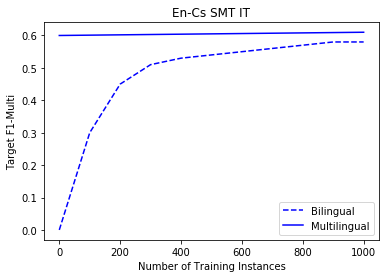
\includegraphics[width=\figlength]{figures/translation_quality_estimation/word_level/en_cs_smt_it.png}
		\caption{En-Cs SMT IT}
		\label{fig:en_cs_smt_results}
	\end{subfigure}
	\begin{subfigure}[b]{\figlength}
		\centering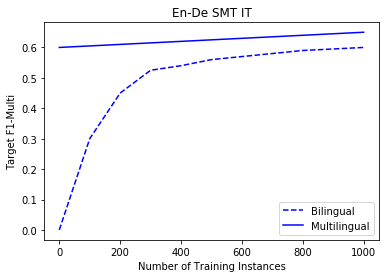
\includegraphics[width=\figlength]{figures/translation_quality_estimation/word_level/en_de_smt_it.png}
		\caption{En-De SMT IT}
		\label{fig:en_de_smt_it_results}
	\end{subfigure}
	\begin{subfigure}[b]{\figlength}
		\centering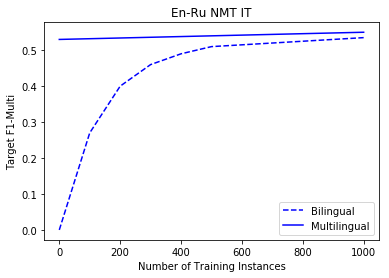
\includegraphics[width=\figlength]{figures/translation_quality_estimation/word_level/en_ru_nmt_it.png}
		\caption{En-Ru NMT IT}
		\label{fig:en_ru_nmt_it_results}
	\end{subfigure}
	\begin{subfigure}[b]{\figlength}
		\centering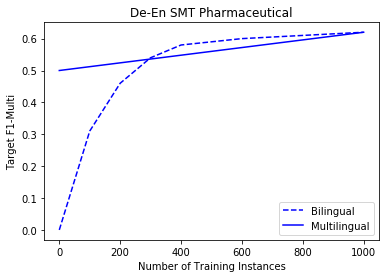
\includegraphics[width=\figlength]{figures/translation_quality_estimation/word_level/de_en_smt_pharm.png}
		\caption{De-En SMT Pharmaceutical}
		\label{fig:de_en_smt_pharm_results}
	\end{subfigure}
	\begin{subfigure}[b]{\figlength}
		\centering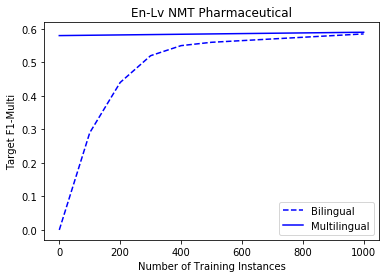
\includegraphics[width=\figlength]{figures/translation_quality_estimation/word_level/en_lv_nmt_pharm.png}
		\caption{En-Lv NMT Pharmaceutical}
		\label{fig:en_lv_nmt_Pharm_results}
	\end{subfigure}
	\begin{subfigure}[b]{\figlength}
		\centering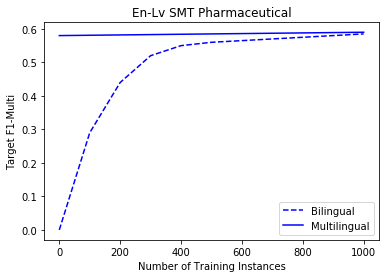
\includegraphics[width=\figlength]{figures/translation_quality_estimation/word_level/en_lv_smt_pharm.png}
		\caption{En-Lv SMT Pharmaceutical}
		\label{fig:en_lv_smt_pharm_results}
	\end{subfigure}
	\begin{subfigure}[b]{\figlength}
		\centering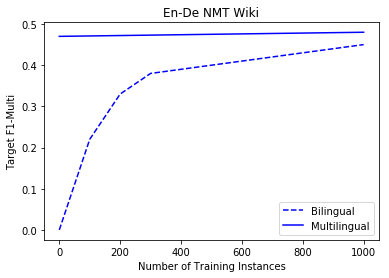
\includegraphics[width=\figlength]{figures/translation_quality_estimation/word_level/en_de_nmt_wiki.png}
		\caption{En-De NMT Wiki}
		\label{fig:en_de_nmt_wiki_results}
	\end{subfigure}
	\begin{subfigure}[b]{\figlength}
		\centering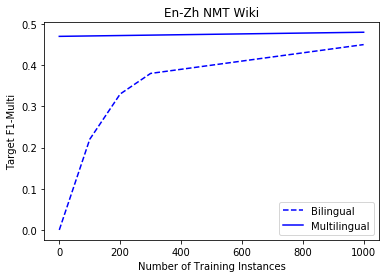
\includegraphics[width=\figlength]{figures/translation_quality_estimation/word_level/en_zh_nmt_wiki.png}
		\caption{En-Zh NMT Wiki}
		\label{fig:en_zh_nmt_wiki_results}
	\end{subfigure}
	\caption{Few-shot learning Results for Word-Level QE. We report Target F1-Multi scores against Number of training instances for multilingual and bilingual models.}
	\label{fig:fewshot_results}
\end{figure}

We also evaluated how the QE models behave with a limited number of training instances. For each language pair, we initiated the weights of the bilingual model with those of the relevant All-1 QE and trained it on 100, 200, 300 and up to 1000 training instances. We compared the results with those obtained having trained the QE model from scratch for that language pair. The results in Figure \ref{fig:fewshot_results} show that All-1 or the multilingual model performs well above the QE model trained from scratch (Bilingual) when there is a limited number of training instances available. Even for the De-En language pair in sentence-level HTER QE and word-level QE, for which we had comparatively poor zero-shot results, the multilingual model provided better results with a few training instances. It seems that having the model weights already fine-tuned in the multilingual model provides an additional boost to the training process which is advantageous in a few-shot scenario.

With these findings we answer our \textbf{RQ3:} multilingual QE models perform better with a limited number of training instances (Few-shot learning) for an unseen language pair in both sentence-level and word-level QE. It is always better to transfer the weights from a multilingual QE model rather than training the weights from scratch for a new language pair.


\section{Conclusion}
\label{sec:multilingual_conclusion}
The traditional way of having a single QE model for each language pair has many limitations; \textit{i. }They need to have annotated training data for each language pair which can be costly, \textit{ii. }Managing several QE models at the same time can be chaotic.  These limitations can hinder the ability of the state-of-the-art QE models to be applied in real-world-applications. As a solution to that we explored multilingual QE with state-of-the-art QE models. We used the sentence-level and word-level QE architectures in \textit{TransQuest} and evaluated them in different multilingual settings. 

In our experiments, we observed that multilingual QE models deliver excellent results on the language pairs they were trained on. In addition, the multilingual QE models perform well in the majority of the zero-shot scenarios where the multilingual QE model is tested on an unseen language pair. Furthermore, multilingual models perform very well with few-shot learning on an unseen language pair when compared to training from scratch for that language pair, proving that multilingual QE models are effective even with a limited number of training instances. This suggests that we can train a single multilingual QE model on as many languages as possible and apply it on other language pairs as well. These findings can be beneficial to perform QE in low-resource languages for which the training data is scarce and when maintaining several QE models for different language pairs is arduous. Considering the benefits of multilingual models, we have released several multilingual sentence-level and word-level pre-trained models on HuggingFace model hub. 

The main limitation of our multilingual evaluation is that all the languages we used throughout the experiments are supported by pre-trained XLM-R model we used. XLM-R large model only supports 100 languages at the moment and there are lot of low resource but common languages like Dzongkha, Tajiki, Tigrinya\footnote{Dzongkha, Tajiki and Tigrinya are the official languages of Bhutan, Tajikistan and Eritrea respectively that are collectively spoken by more than 18 million people in the world} etc that are not supported by XLM-R. A question can arise about how the language pairs that are not supported by XLM-R perform in our multilingual QE environment. However, as far as we know, until very recently, there were no annotated QE datasets either for the languages outside the 100 languages supported by XLM-R. Therefore, it would not be possible to carry out a proper evaluation. Very recently in WMT 2021, an annotated QE dataset for Pashto-English and Khmer-English was introduced. Pashto and Khmer are not supported by XLM-R at the moment and it would be interesting to experiment them with our multilingual models which we hope to do in future work.

Pre-trained multilingual transformer models are rapidly increasing popularity in NLP community. From them, one notable multilingual transformer model is mT5 \autocite{xue-etal-2021-mt5}; multilingual text to text transformer model which considers every task as a sequence to sequence task. It has provided very good results in variety of multilingual NLP tasks. As future work, we hope to incorporate mT5 in \textit{TransQuest} framework and evaluate it in a multilingual QE environment.


